\documentclass[12pt,a4paper]{article}

% Pacotes essenciais
\usepackage[utf8]{inputenc}
\usepackage[portuguese]{babel}
\usepackage{amsmath}
\usepackage{amsfonts}
\usepackage{amssymb}
\usepackage{graphicx}
\usepackage{geometry}
\usepackage{hyperref}
\usepackage{float}
\usepackage{booktabs} % Para tabelas de alta qualidade tipográfica

\geometry{left=2.5cm, right=2.5cm, top=3cm, bottom=3cm}

\title{Trabalho-Prova (P1) - Inteligência Artificial \\ \large Resolução e Relatório Técnico}
\author{Gabriel Martins Brum}
\date{\today}

\begin{document}

\maketitle

\tableofcontents
\newpage

% ==========================================
% QUESTÃO 1
% ==========================================
\section{Definição e Exploração do Conjunto de Dados}

\subsection{Seleção da Base de Dados}
O conjunto de dados selecionado para o presente trabalho designa-se \textbf{Credit Card Fraud Detection}, disponibilizado publicamente no repositório Kaggle.

\textbf{Endereço eletrónico da base de dados:} \url{https://www.kaggle.com/datasets/mlg-ulb/creditcardfraud/}

\subsection{Atributos Preditivos e Variável Alvo}
O \textit{dataset} engloba registos de transações efetuadas através de cartões de crédito, sendo caracterizado pela seguinte estrutura de dados:
\begin{itemize}
    \item \textbf{Atributos Preditivos (Entradas):} Por imperativos de confidencialidade bancária, as características originais (\textit{features}) foram previamente submetidas a uma Análise de Componentes Principais (PCA), originando um vetor de 28 variáveis contínuas ($V1, V2, \dots, V28$). As únicas variáveis independentes não transformadas são o \textit{Time} (tempo decorrido em segundos entre transações) e o \textit{Amount} (montante monetário da transação).
    \item \textbf{Variável Alvo (Saída):} A variável categórica \textit{Class}, que assume o valor $1$ para anomalias (transações fraudulentas) e $0$ para observações normais (transações legítimas).
\end{itemize}

\subsection{Motivação e Relevância}
A seleção deste problema justifica-se pelo desafio técnico inerente à modelação preditiva em contextos de classes com distribuição fortemente assimétrica (desbalanceamento severo). Este cenário é paradigmático e de criticidade extrema no setor financeiro, exigindo técnicas rigorosas de pré-processamento e métricas de avaliação robustas para a viabilização de sistemas de deteção de anomalias em ambiente de produção.

% ==========================================
% QUESTÃO 2
% ==========================================
\section{Abordagem Metodológica e Avaliação de Modelos}

Para a tarefa de classificação binária, selecionaram-se três algoritmos com complexidades arquitetónicas distintas, permitindo uma análise comparativa e evolutiva do desempenho. A otimização dos hiperparâmetros foi conduzida através de uma pesquisa estocástica no espaço de parâmetros (\textit{Randomized Search Cross-Validation}), configurada com 10 iterações (\texttt{n\_iter=10}) e validação cruzada de 3 partições (\texttt{cv=3}), adotando-se a métrica F1-Score como critério de otimização.

Os espaços de pesquisa e as configurações ótimas identificadas para cada estimador são detalhados de seguida:

\begin{enumerate}
    \item \textbf{Regressão Logística (Baseline):} Adotado como modelo linear de referência pela sua interpretabilidade e eficiência computacional. O espaço de pesquisa avaliou os algoritmos de otimização \texttt{liblinear} e \texttt{saga}, com aplicação de penalizações de regularização $L1$ e $L2$, variando o inverso da força de regularização ($C$) no intervalo $[0.01, 0.1, 1, 10, 100]$.
    \begin{itemize}
        \item \textbf{Configuração ótima:} \texttt{solver='liblinear'}, \texttt{penalty='l1'}, \texttt{C=100}.
    \end{itemize}

    \item \textbf{Random Forest:} Algoritmo baseado no método de \textit{ensemble} do tipo \textit{bagging}, reconhecido pela sua resiliência perante o sobreajuste (\textit{overfitting}). O espaço hiperparamétrico abrangeu o número de estimadores (\texttt{n\_estimators} entre 100 e 300), o limite de profundidade das árvores (\texttt{max\_depth}), o critério de divisão de nós (\texttt{min\_samples\_split}) e a heurística de seleção de atributos (\texttt{max\_features}).
    \begin{itemize}
        \item \textbf{Configuração ótima:} \texttt{n\_estimators=300}, \texttt{max\_depth=30}, \texttt{min\_samples\_split=5}, \texttt{max\_features='log2'}.
    \end{itemize}

    \item \textbf{XGBoost:} Algoritmo avançado fundamentado em \textit{Gradient Boosting}, frequentemente considerado o estado da arte para dados tabulares. A calibração focou-se na contenção da variância e na prevenção da memorização de instâncias sintéticas geradas pelo SMOTETomek, explorando a taxa de aprendizagem (\texttt{learning\_rate}), a profundidade máxima (\texttt{max\_depth}), e parâmetros de subamostragem (\texttt{subsample} e \texttt{colsample\_bytree}).
    \begin{itemize}
        \item \textbf{Configuração ótima:} \texttt{n\_estimators=200}, \texttt{max\_depth=7}, \texttt{learning\_rate=0.2}, \texttt{subsample=0.8}, \texttt{colsample\_bytree=0.8}.
    \end{itemize}
\end{enumerate}

\subsection{Resultados e Métricas de Avaliação}

\subsubsection{Fundamentação das Métricas}
Em conjuntos de dados afetados por desbalanceamento severo, a métrica de Exatidão (\textit{Accuracy}) revela-se enviesada (todos os modelos apresentaram exatidão $\ge 99\%$, camuflando a taxa real de erros na classe minoritária). Consequentemente, a avaliação analítica pautou-se por:
\begin{itemize}
    \item \textbf{Revocação (\textit{Recall} / Sensibilidade):} Capacidade do classificador em identificar a totalidade das fraudes reais, minimizando os Falsos Negativos.
    \item \textbf{Precisão (\textit{Precision}):} Fiabilidade das predições positivas do modelo, reduzindo a incidência de Falsos Positivos.
    \item \textbf{F1-Score:} A média harmónica entre a Precisão e a Revocação, instituída como métrica global de ordenação da eficácia dos algoritmos.
\end{itemize}

\subsubsection{Análise de Desempenho e Matrizes de Confusão}
A inferência no conjunto de teste (composto por 56.864 instâncias normais e 98 fraudes intrínsecas) evidenciou a seguinte progressão técnica:

\vspace{0.5cm}
\textbf{1. Regressão Logística} \\
Apesar de exibir uma excelente Revocação (0.90), denotando a deteção de $90\%$ das fraudes, o modelo revelou extrema fragilidade na Precisão (0.13), culminando num \textbf{F1-Score de apenas 0.23}. A matriz de confusão demonstra que, operacionalmente, o classificador incorre num rácio insustentável de falsos alarmes: para identificar 88 transações fraudulentas (Verdadeiros Positivos), o modelo bloqueou indevidamente 570 transações legítimas (Falsos Positivos).
\begin{figure}[H]
    \centering
    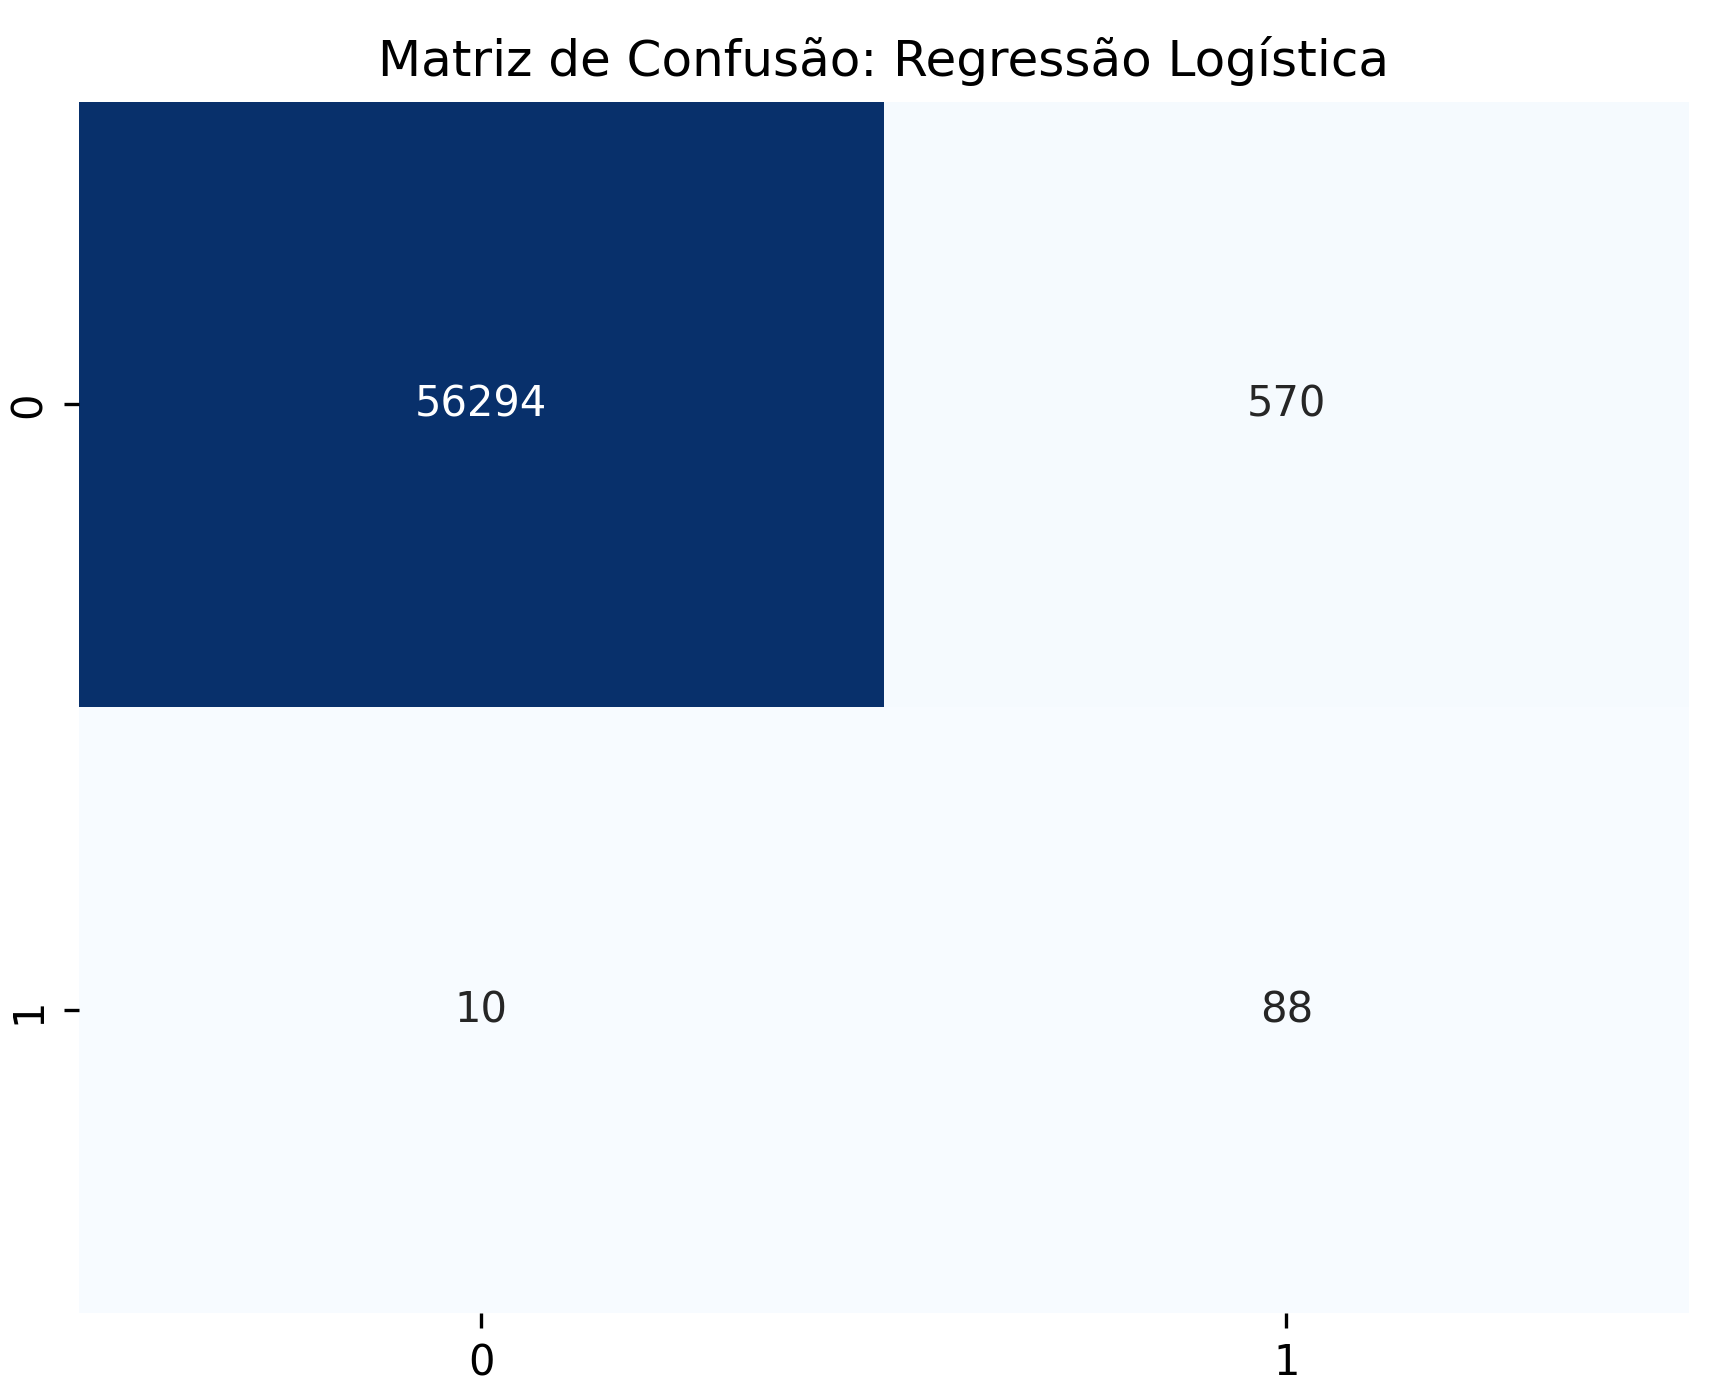
\includegraphics[width=0.5\textwidth]{img/matriz_confusao_rl.png}
    \caption{Matriz de Confusão - Regressão Logística}
\end{figure}

\vspace{0.5cm}
\textbf{2. Random Forest} \\
Observou-se um incremento substancial do desempenho preditivo, materializado num \textbf{F1-Score de 0.84}. Este método conseguiu equalizar a Precisão e a Revocação em 0.84, demonstrando elevada resiliência face ao ruído de amostragem. O modelo identificou 82 fraudes reais, restringindo drasticamente os Falsos Positivos para apenas 16 instâncias.
\begin{figure}[H]
    \centering
    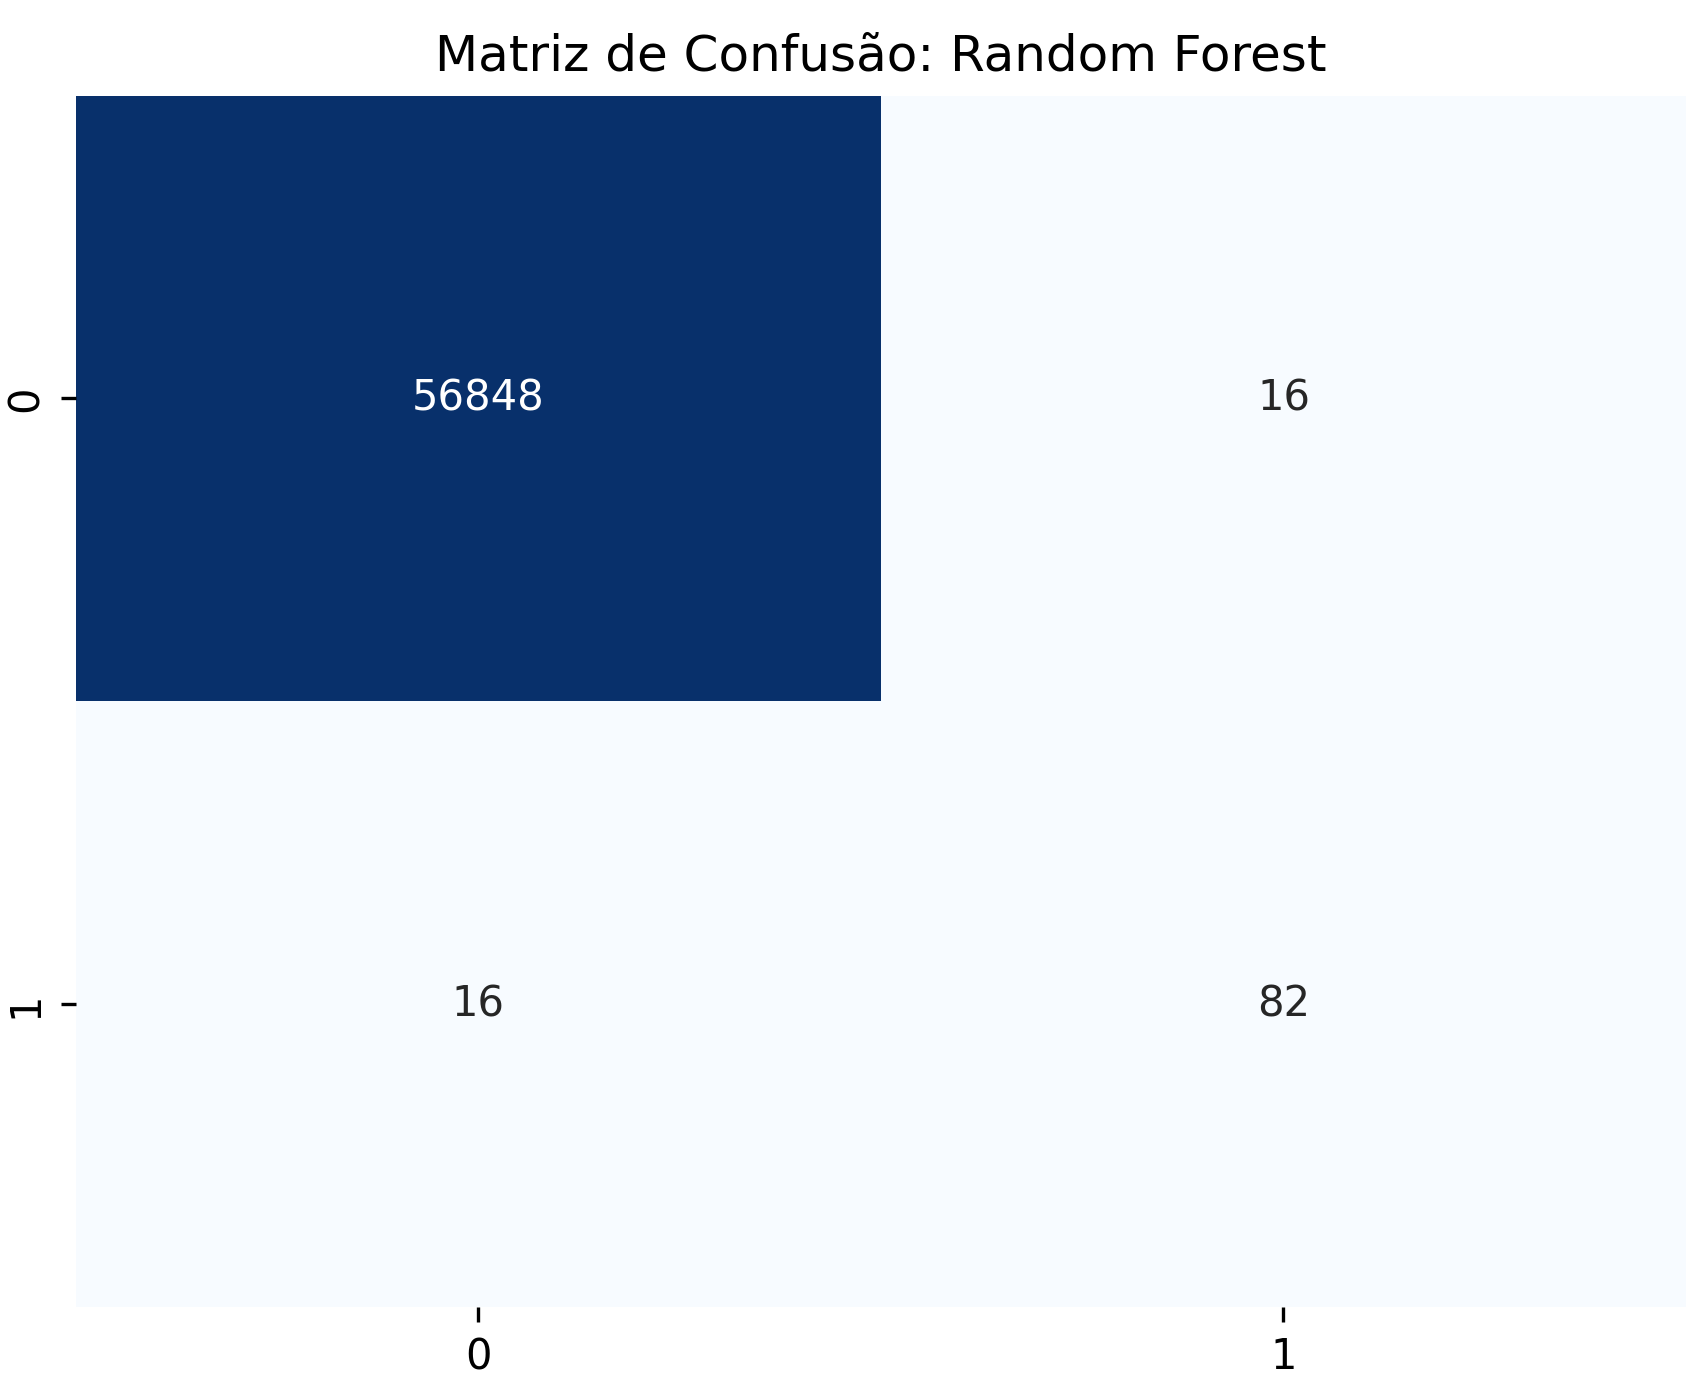
\includegraphics[width=0.5\textwidth]{img/matriz_confusao_rf.png}
    \caption{Matriz de Confusão - Random Forest}
\end{figure}

\vspace{0.5cm}

\textbf{3. XGBoost} \\
Este algoritmo obteve o desempenho superior nesta experimentação, alcançando um \textbf{F1-Score de 0.85}. A sua capacidade de generalização superou marginalmente a da Random Forest, registando 0.85 de Precisão e 0.86 de Revocação. A fronteira de decisão capturou 84 fraudes e conteve os Falsos Positivos em 15 transações.
\begin{figure}[H]
    \centering
    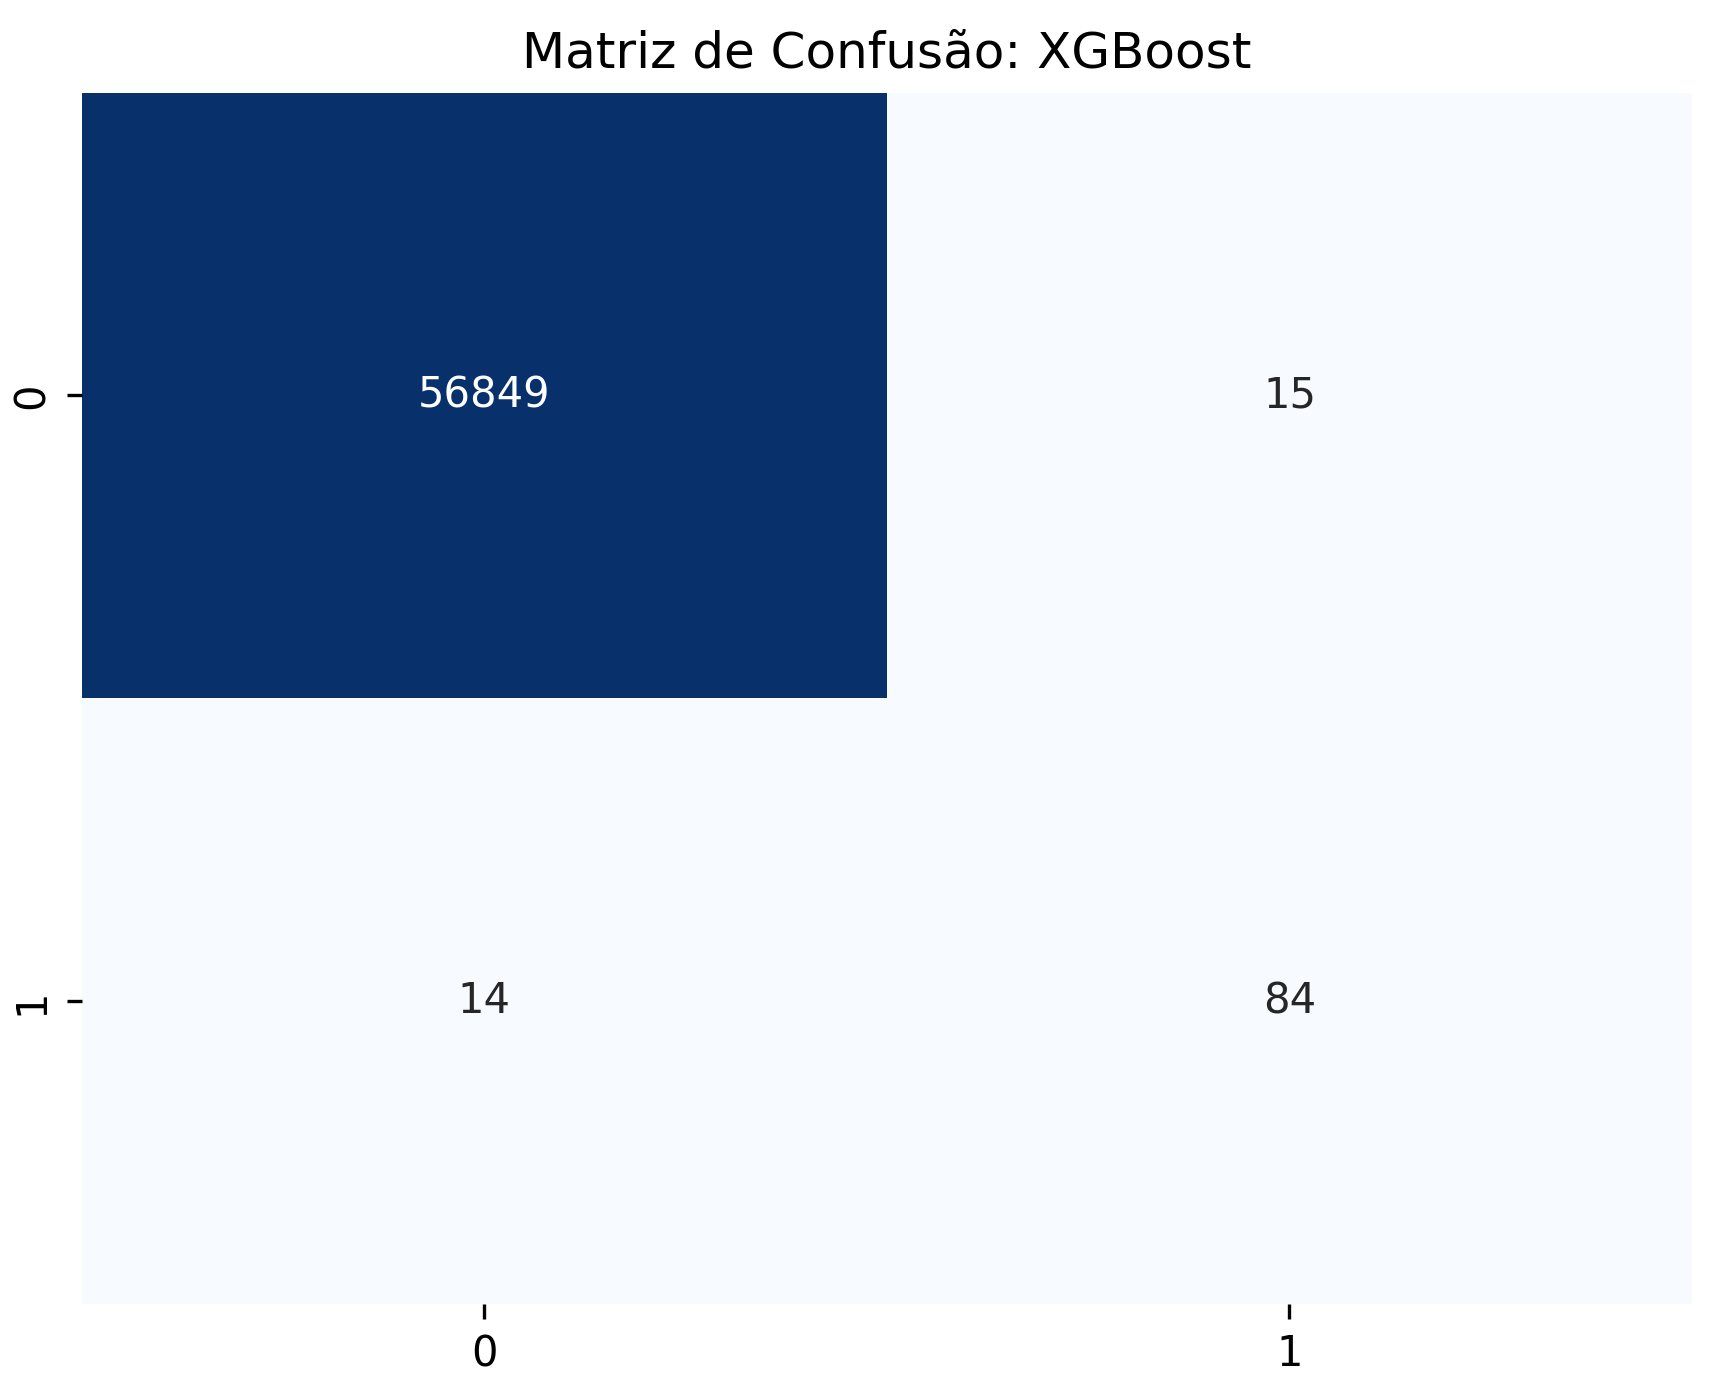
\includegraphics[width=0.5\textwidth]{img/matriz_confusao_xgb.png}
    \caption{Matriz de Confusão - XGBoost}
\end{figure}

A análise de importância de atributos (\textit{Feature Importance}) sublinhou a relevância da variável temporal (\textit{Time}) no processo decisório do XGBoost, seguida pela proeminência de componentes principais específicas, nomeadamente V14, V4 e V16 (conforme patente na Figura 4).
\begin{figure}[H]
    \centering
    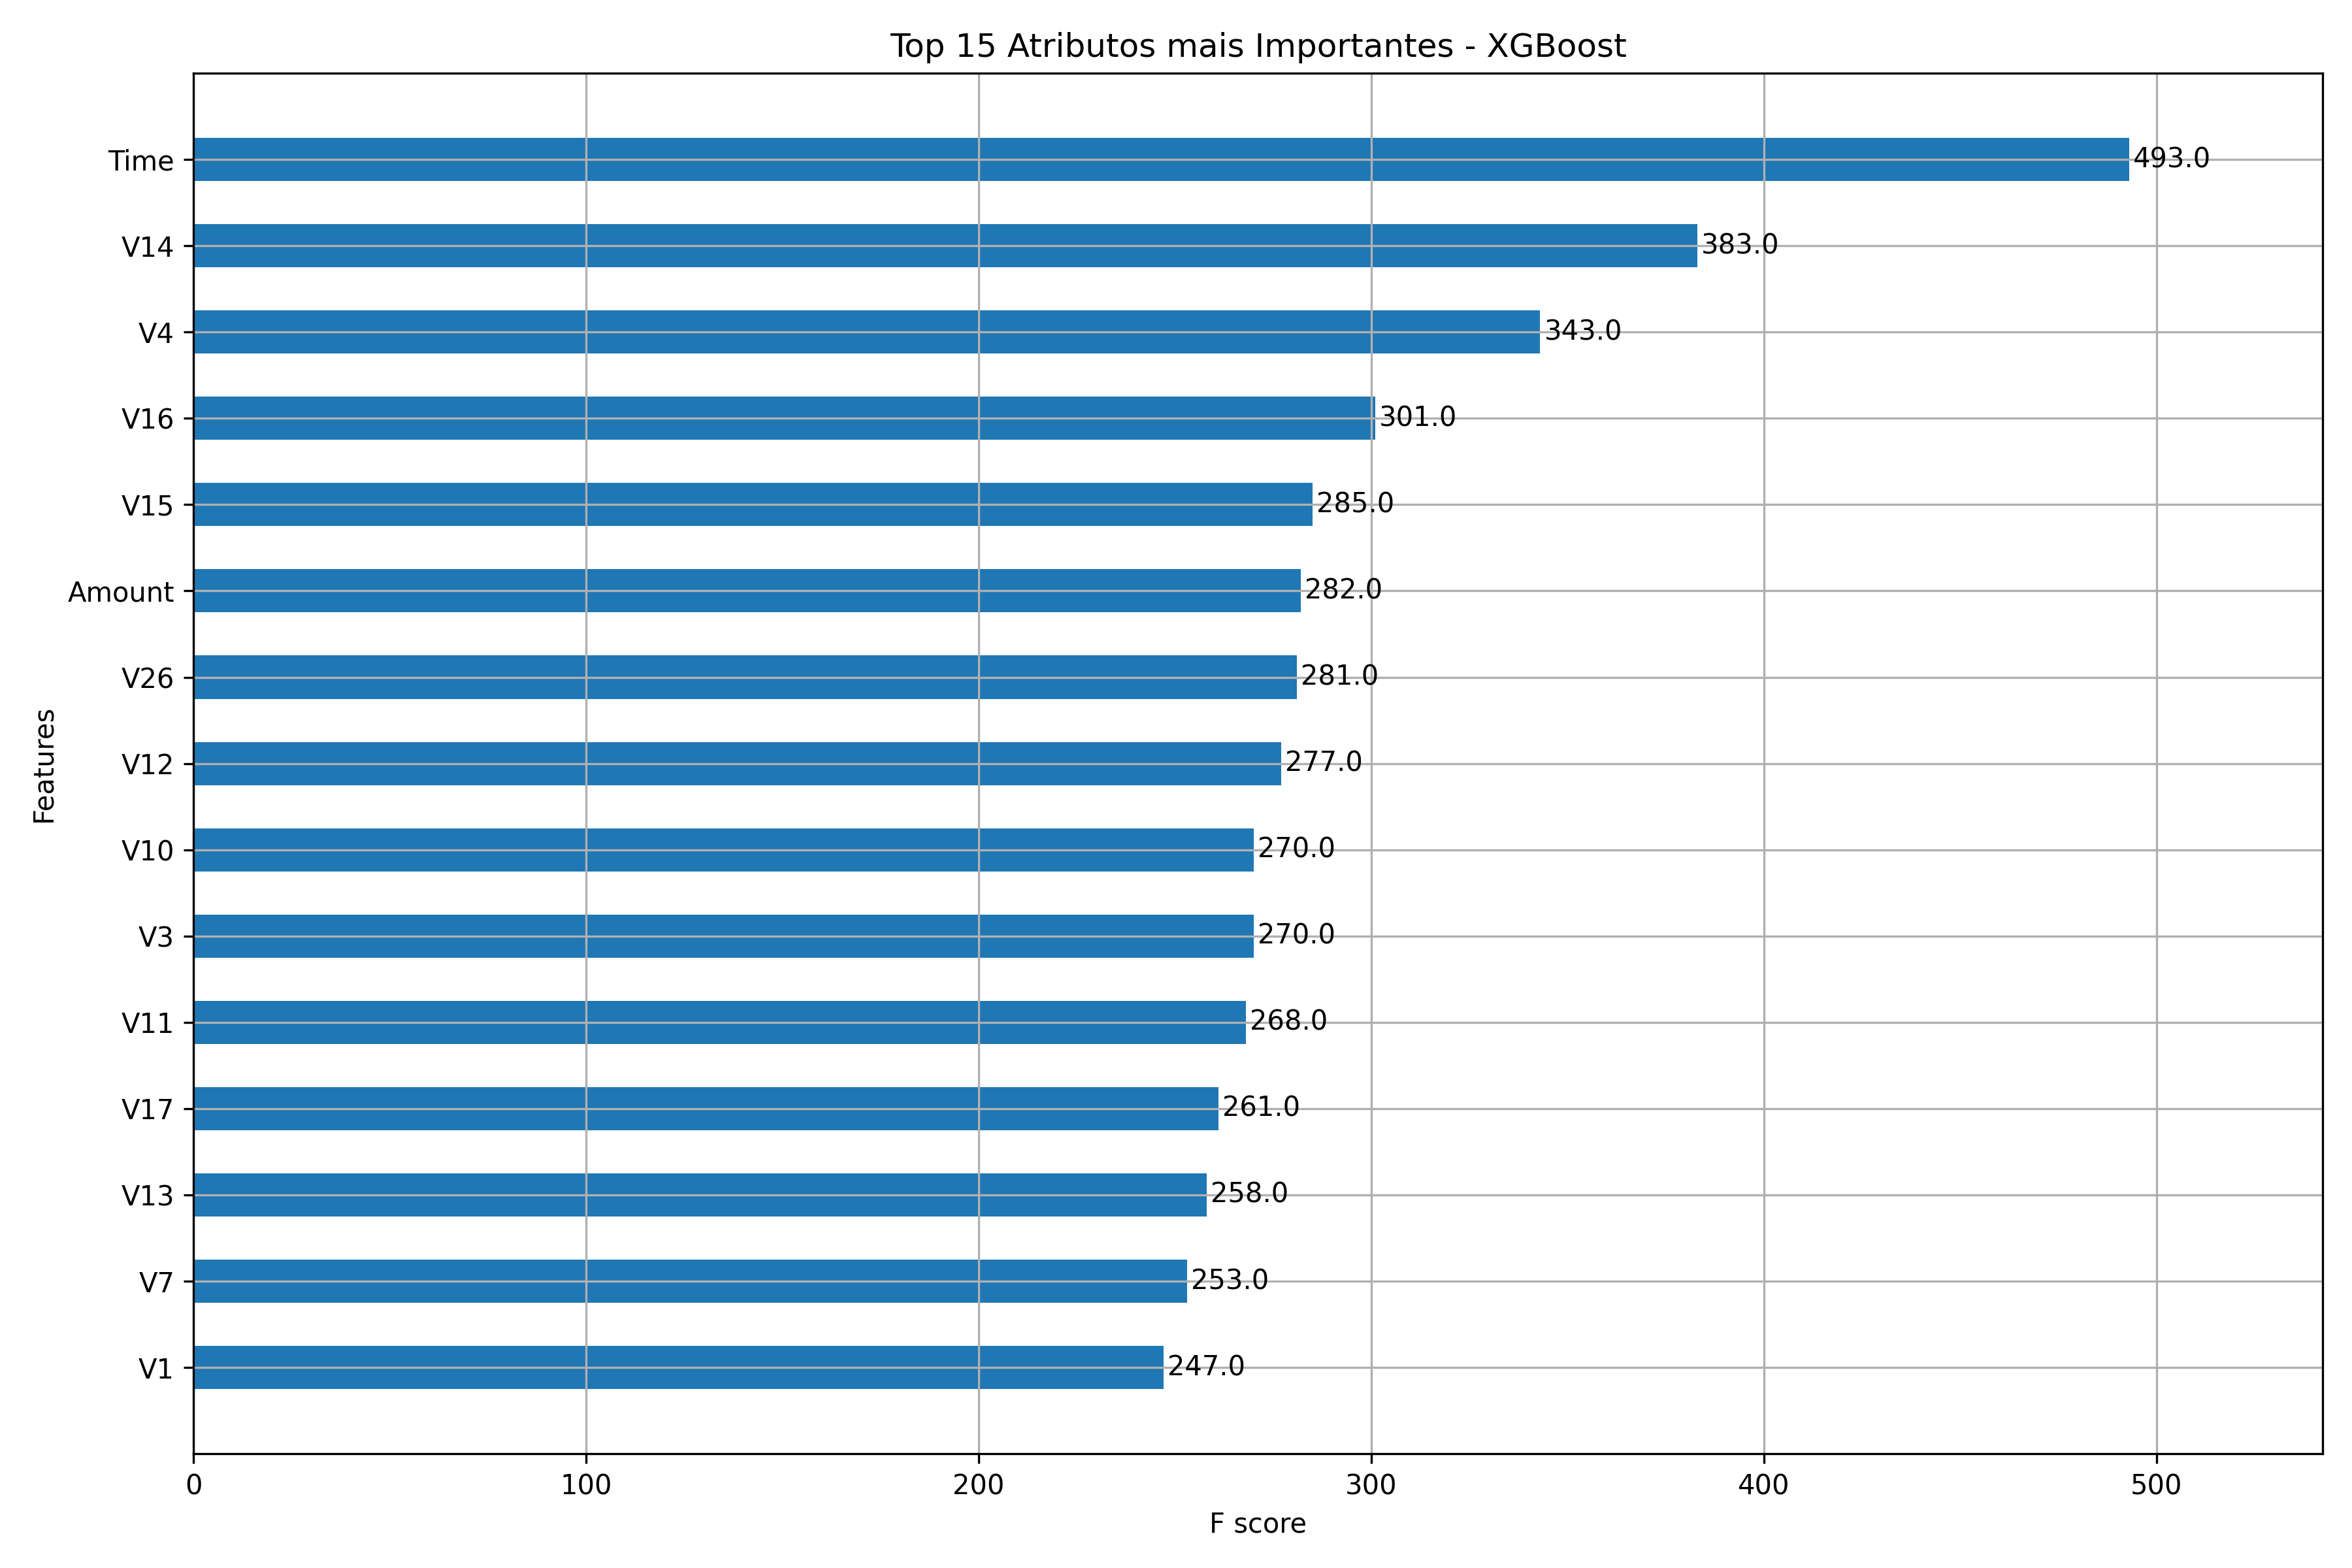
\includegraphics[width=1.1\textwidth]{img/feature_importance_xgb.png}
    \caption{Importância Relativa dos Atributos (\textit{Feature Importance}) - XGBoost}
\end{figure}

\subsubsection{Estudo Comparativo e Análise da Curva Precision-Recall}
A avaliação comparativa corrobora o ganho informacional obtido através de métodos não-lineares de \textit{Ensemble} (Random Forest e XGBoost) em detrimento de modelos lineares estritos (Regressão Logística) para o tratamento de distribuições com assimetria severa.

Para aprofundar a avaliação reportada nas matrizes de confusão, a Figura 5 ilustra a \textbf{Curva Precision-Recall (PR)}, que traduz a flutuação do desempenho sob diferentes limiares de decisão (\textit{thresholds}). O gráfico explicita o compromisso (\textit{trade-off}) estatístico: a maximização absoluta do \textit{Recall} exige uma atenuação dos critérios de predição, o que invariavelmente induz uma degradação da \textit{Precision}.

A \textbf{Regressão Logística} revelar-se-ia inadequada num sistema financeiro real. Com uma precisão limiar de $13\%$, os 570 Falsos Positivos gerados comprometem gravemente a qualidade do serviço, traduzindo-se num rácio aproximado de 6,5 clientes legítimos bloqueados para cada fraude evitada. A Curva PR evidencia esta limitação estrutural (linha azul): verifica-se um declínio acentuado da Precisão na fase inicial da curva, provando a ineficácia do modelo na segregação das classes.

A adoção do modelo \textbf{Random Forest} mitigou eficientemente o impacto do ruído introduzido pelo sobredimensionamento sintético da amostra (SMOTETomek). Ao restringir a expansão das árvores (\texttt{max\_depth=30}), ocorreu uma redução dos Falsos Positivos de uma magnitude de centenas para apenas 16. A estabilidade desta arquitetura reflete-se na Curva PR (linha laranja), mantendo uma Precisão expressiva e constante mesmo em limiares calibrados para capturar uma elevada taxa de fraudes.

Conclusivamente, o \textbf{XGBoost} provou ser a ferramenta preditiva mais robusta, exibindo a trajetória mais resiliente na curva (linha verde) e um excelente balanço entre as métricas. Ao refinar iterativamente as fragilidades das árvores predecessoras mediante otimização por gradiente, a fronteira de decisão convergiu para o ponto ótimo: identificação de 84 das 98 fraudes intrínsecas ao conjunto de teste, ao mesmo tempo em que conteve de forma rigorosa os alarmes falsos (apenas 15 num universo inferencial de 56.864 instâncias normais). No paradigma de negócio, este \textit{gradient booster} garante o compromisso ótimo entre a mitigação do risco de crédito (falsos negativos) e a preservação da experiência do consumidor.

\begin{figure}[H]
    \centering
    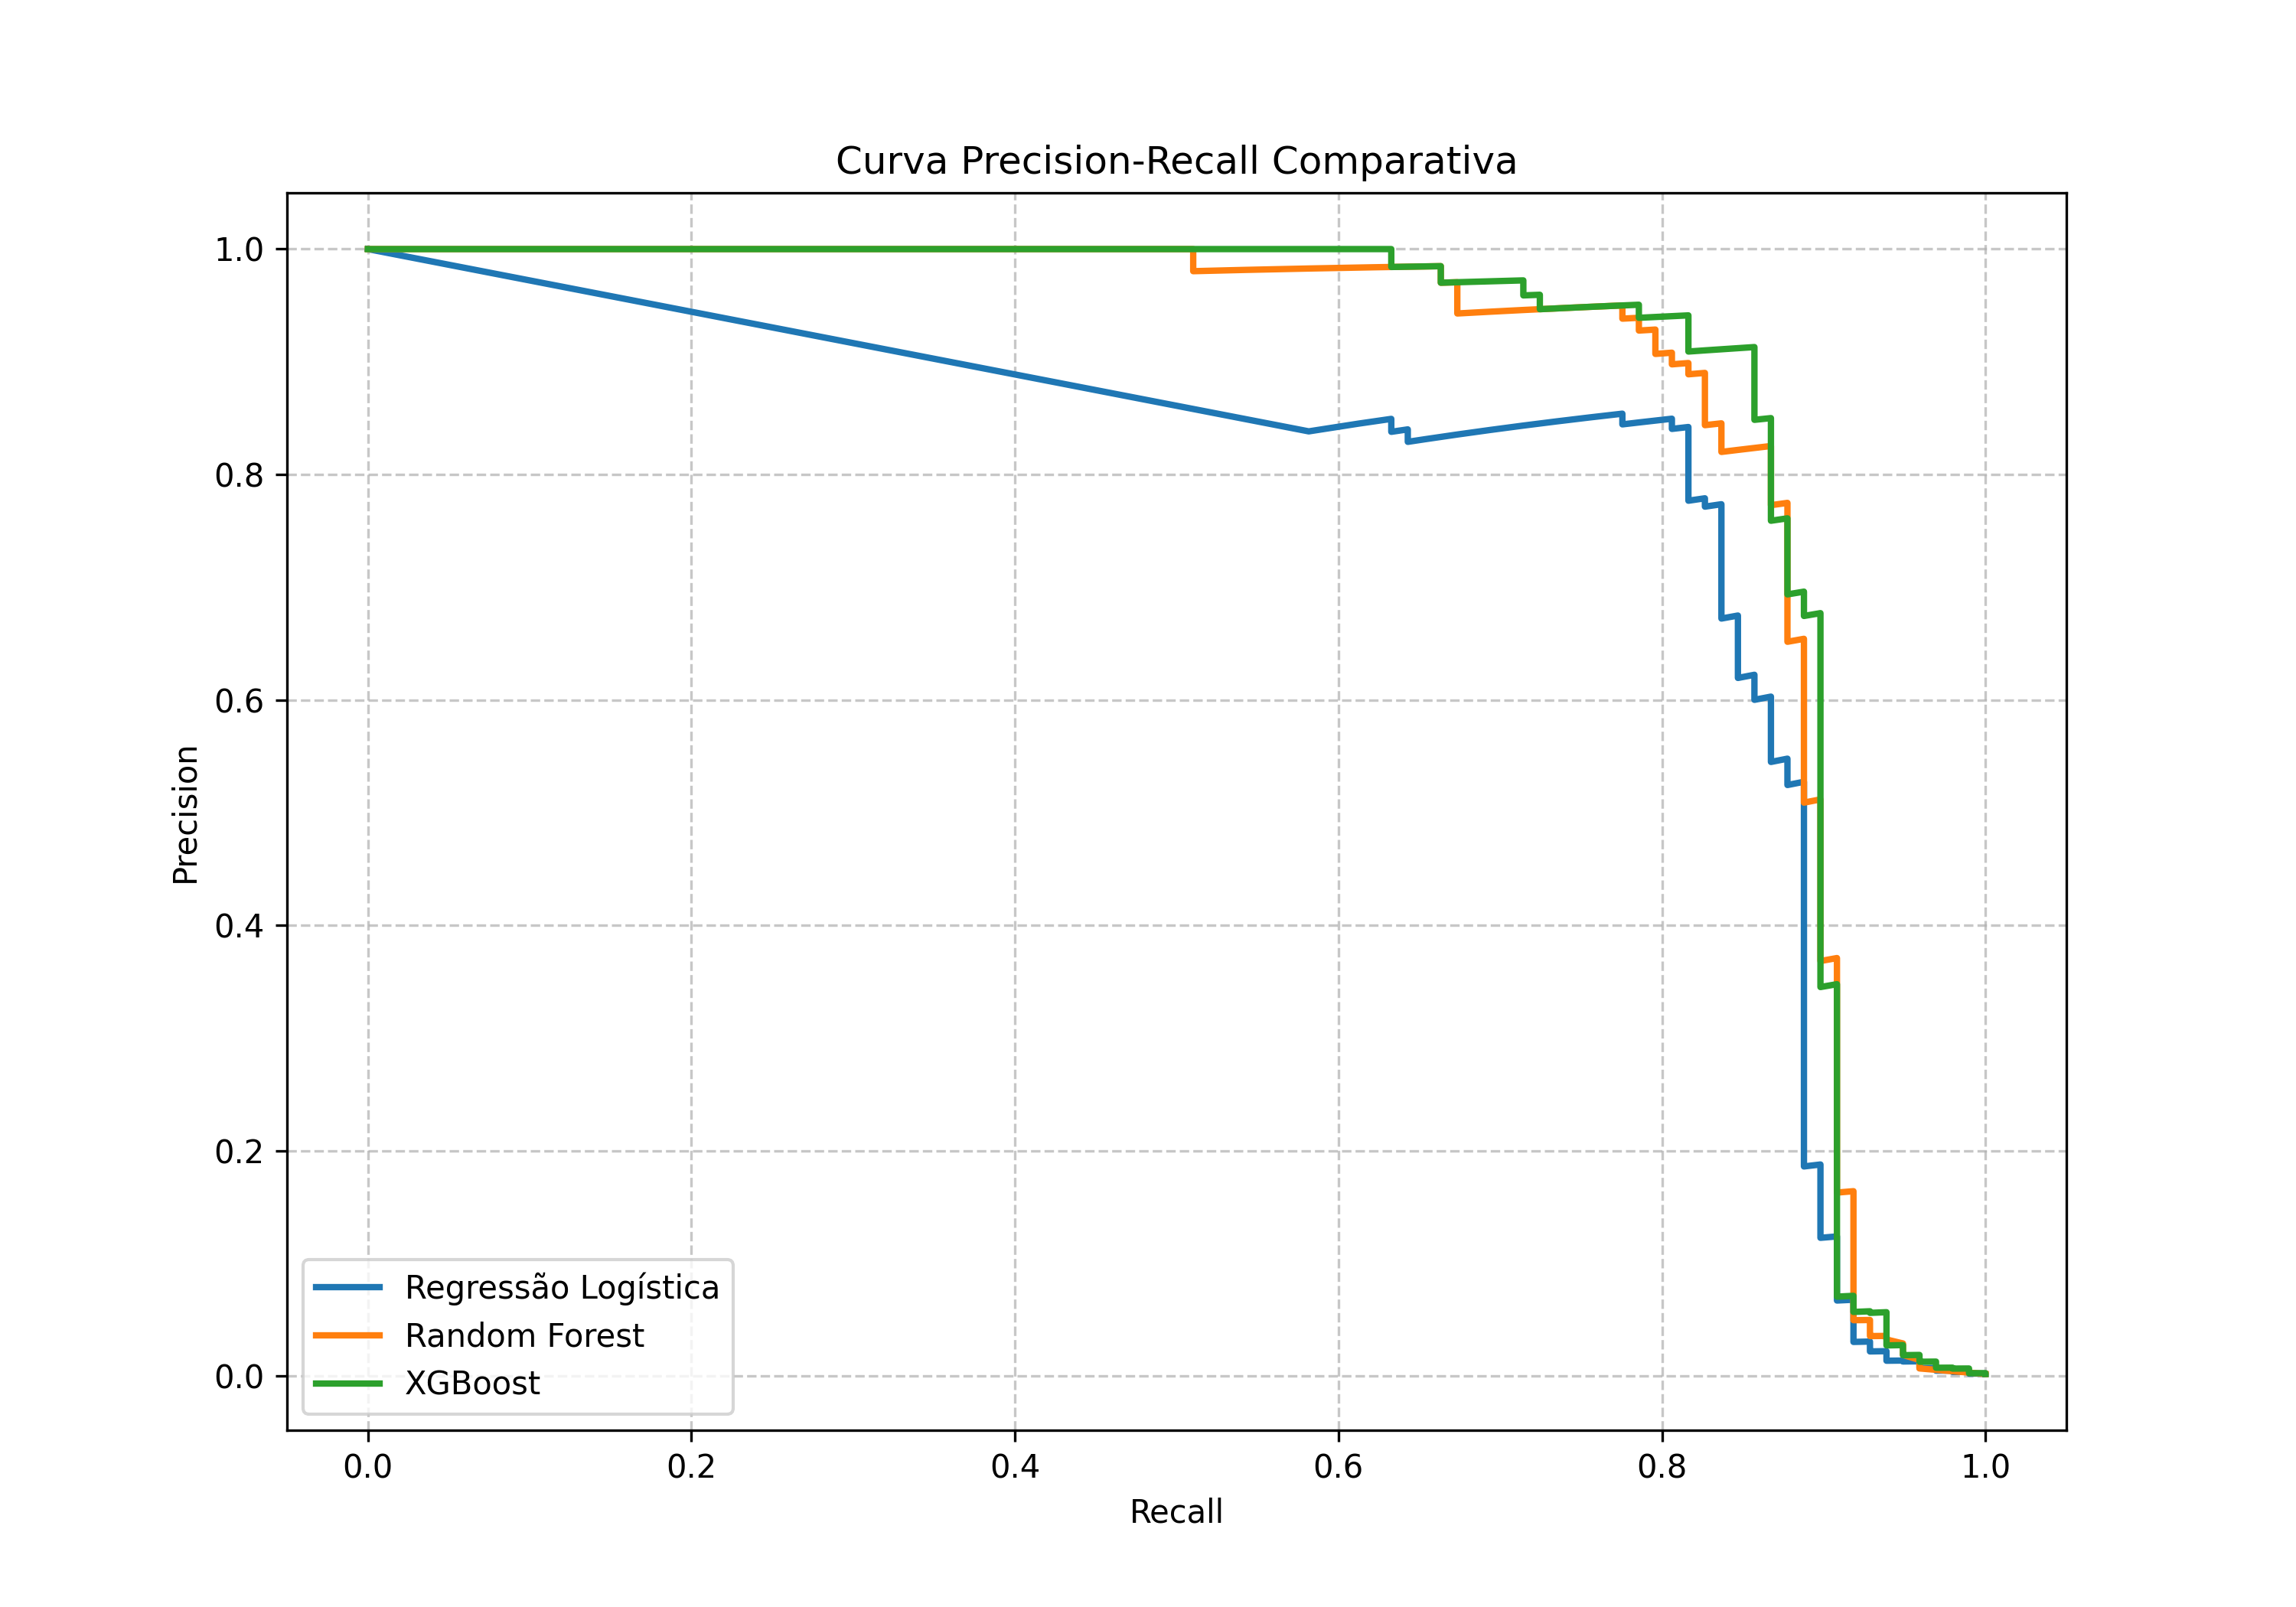
\includegraphics[width=1\textwidth]{img/curva_precision_recall.png}
    \caption{Curva \textit{Precision-Recall} documentando o \textit{trade-off} de performance consoante o limiar de probabilidade adotado.}
\end{figure}
% ==========================================
% QUESTÃO 3
% ==========================================
\section{Análise da Base Breast Cancer Wisconsin}

Esta secção utiliza o \textit{dataset} disponível na biblioteca \texttt{scikit-learn} (\texttt{load\_breast\_cancer}), focado no diagnóstico de tumores mamários.

\subsection{Análise de Outliers}
Para a análise de valores atípicos (\textit{outliers}), foram selecionadas as variáveis contínuas \texttt{mean area} (área média do tumor) e \texttt{mean compactness} (compacidade média). A Figura abaixo apresenta os \textit{boxplots} gerados.

\begin{figure}[H]
    \centering
    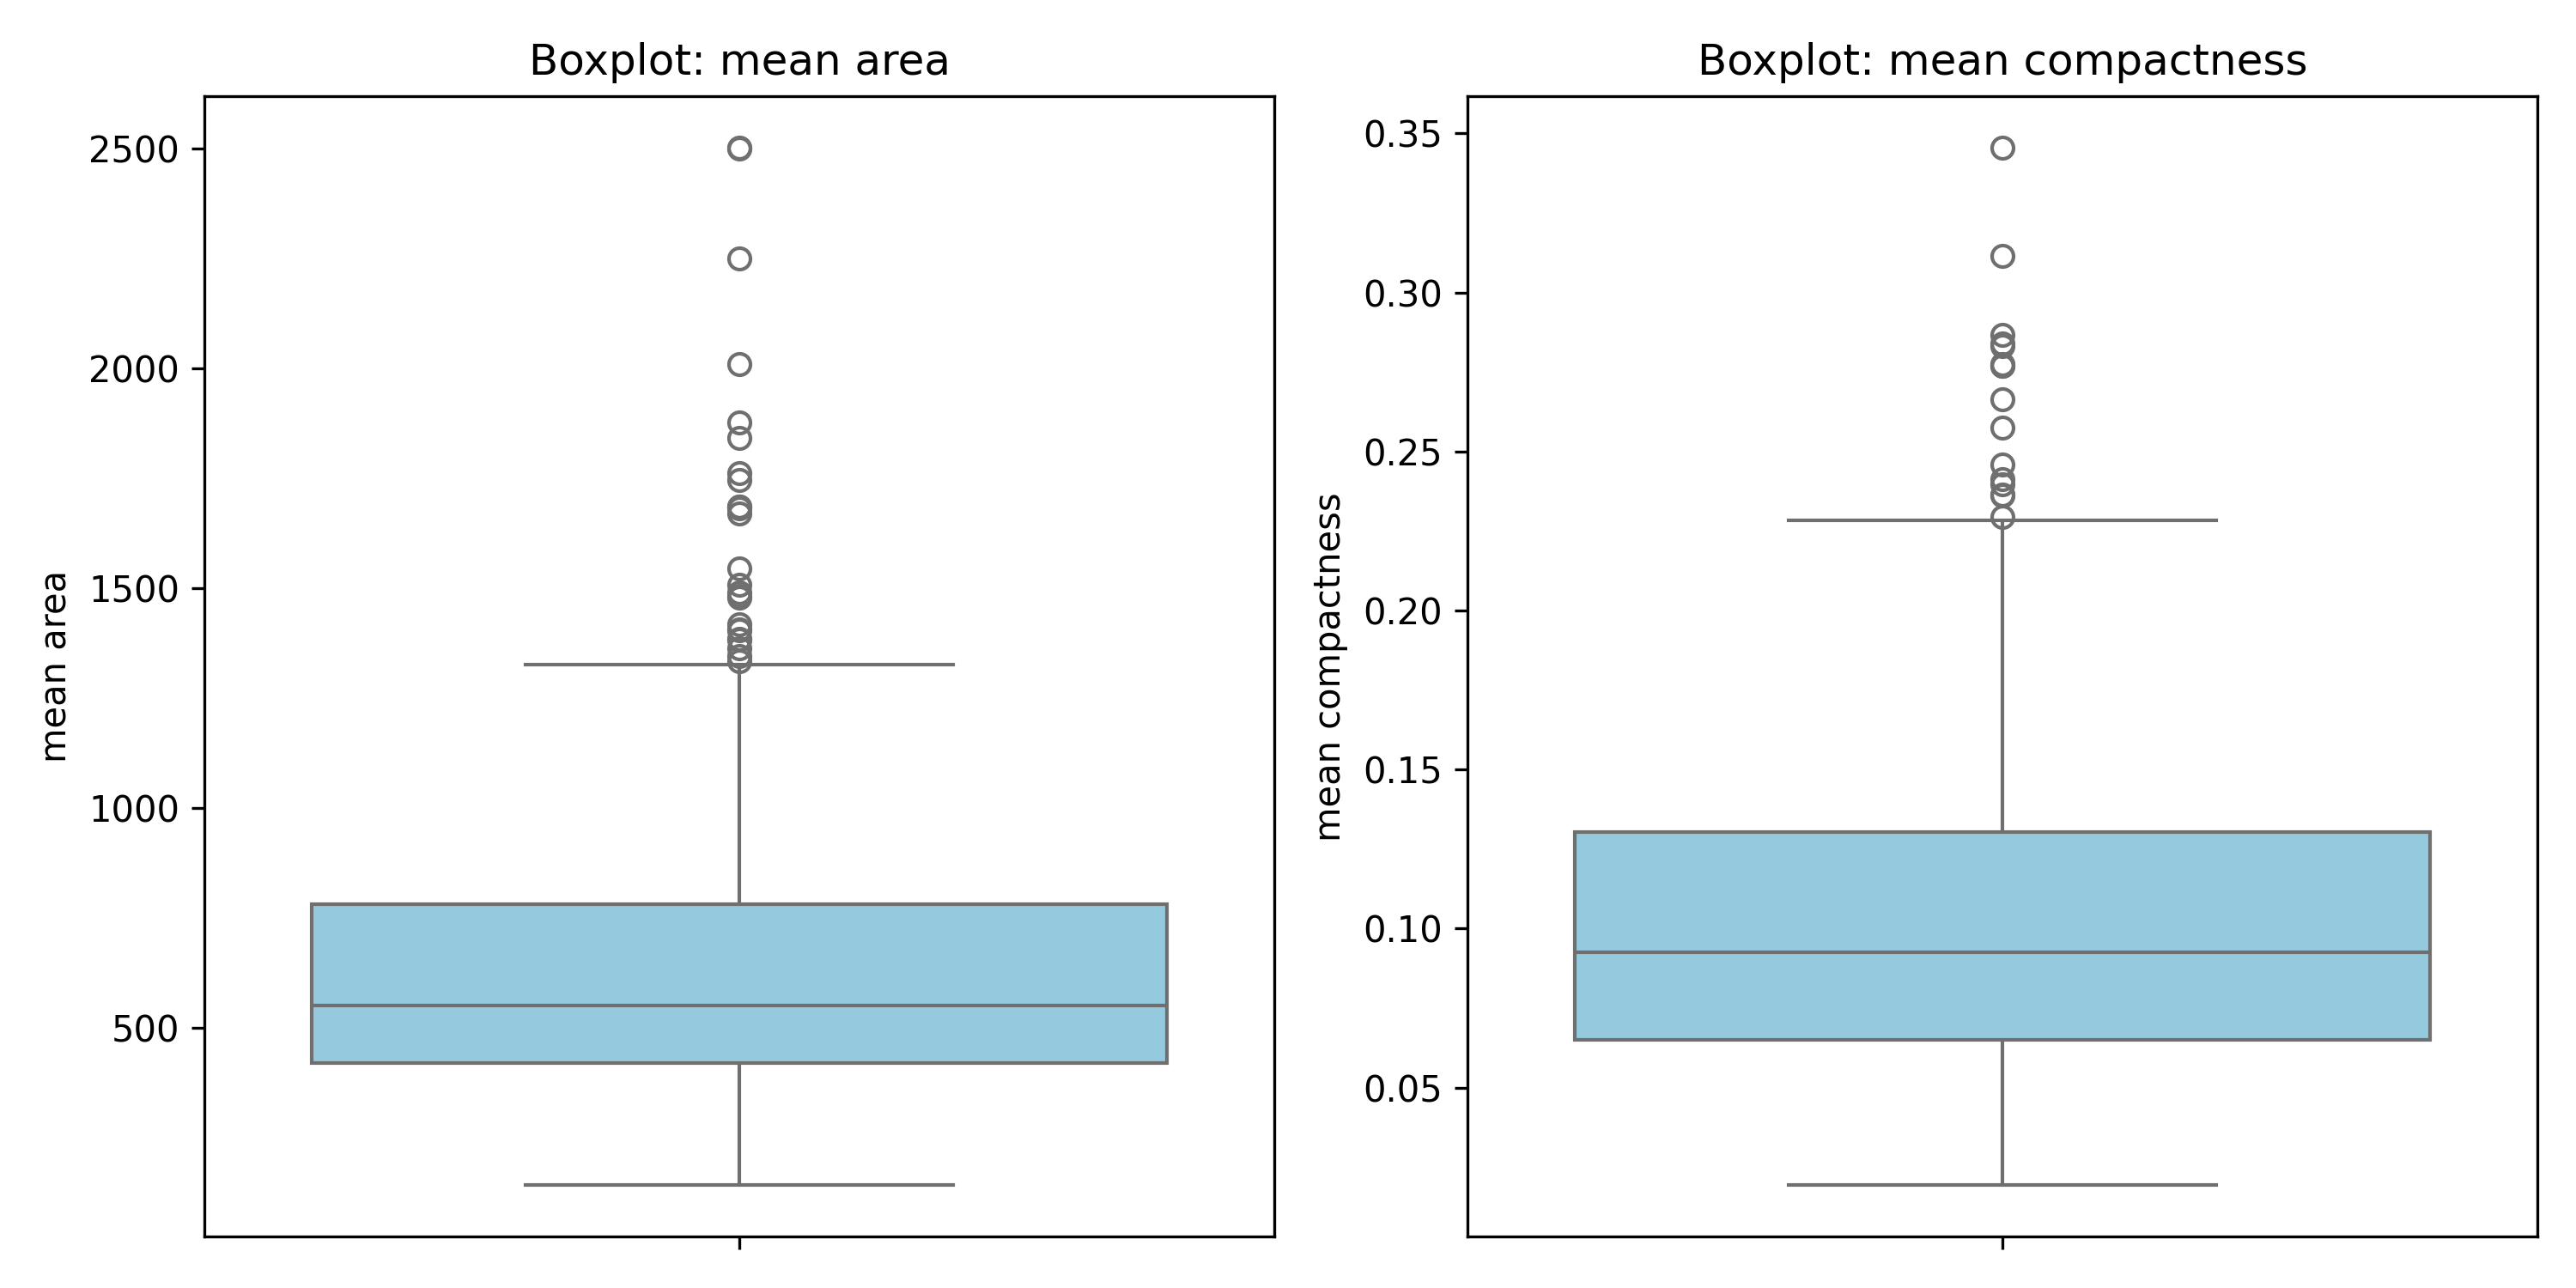
\includegraphics[width=1\textwidth]{img/boxplots_outliers.png}
    \caption{Análise de distribuição e \textit{outliers} para variáveis contínuas.}
\end{figure}

É notória a presença de múltiplos \textit{outliers} na cauda superior de ambas as distribuições (representados pelos pontos acima do limite superior do bigode do \textit{boxplot}).

\textbf{Impacto nos modelos:} A presença destes \textit{outliers} tem um impacto crítico e assimétrico consoante a arquitetura do algoritmo de Aprendizado de Máquina. 
Em modelos baseados no cálculo de distâncias (como KNN, \textit{K-Means} ou \textit{Support Vector Machines}) ou modelos lineares baseados na minimização do erro quadrático (como a Regressão Logística ou Linear clássica), os \textit{outliers} distorcem severamente as fronteiras de decisão, pois os algoritmos tentam ajustar-se a esses valores extremos, degradando a capacidade de generalização. Em contrapartida, algoritmos baseados em árvores de decisão (como \textit{Random Forest} ou XGBoost) são naturalmente imunes a estas anomalias, visto que as divisões dos nós (\textit{splits}) dependem apenas da ordenação dos valores e não das distâncias absolutas entre eles.

\subsection{Matriz de Correlação e Multicolinearidade}
A matriz de correlação calculada (medida pelo coeficiente de Pearson) revelou associações lineares de fortíssima magnitude entre as características morfométricas do tumor.

\textbf{Multicolinearidade:} Existem indícios claríssimos de multicolinearidade estrutural no \textit{dataset}. Os resultados computacionais demonstraram que variáveis derivadas da mesma dimensão espacial partilham praticamente a mesma informação. As maiores correlações encontradas foram:
\begin{itemize}
    \item \texttt{mean radius} e \texttt{mean perimeter}: Correlação de $0.9979$
    \item \texttt{worst radius} e \texttt{worst perimeter}: Correlação de $0.9937$
    \item \texttt{mean radius} e \texttt{mean area}: Correlação de $0.9874$
\end{itemize}
A inclusão simultânea destas variáveis pode prejudicar algoritmos lineares, causando instabilidade na estimação dos coeficientes preditivos (redundância informacional).

\textbf{Associação com o Diagnóstico:} O \textit{dataset} utiliza a codificação onde 0 representa "Maligno" e 1 "Benigno". A análise demonstrou que as variáveis mais associadas à predição correta do diagnóstico são referentes ao "pior" estado (\textit{worst}) das células: \texttt{worst concave points} (0.7936), \texttt{worst perimeter} (0.7829) e \texttt{worst radius} (0.7765).

\begin{figure}[H]
    \centering
    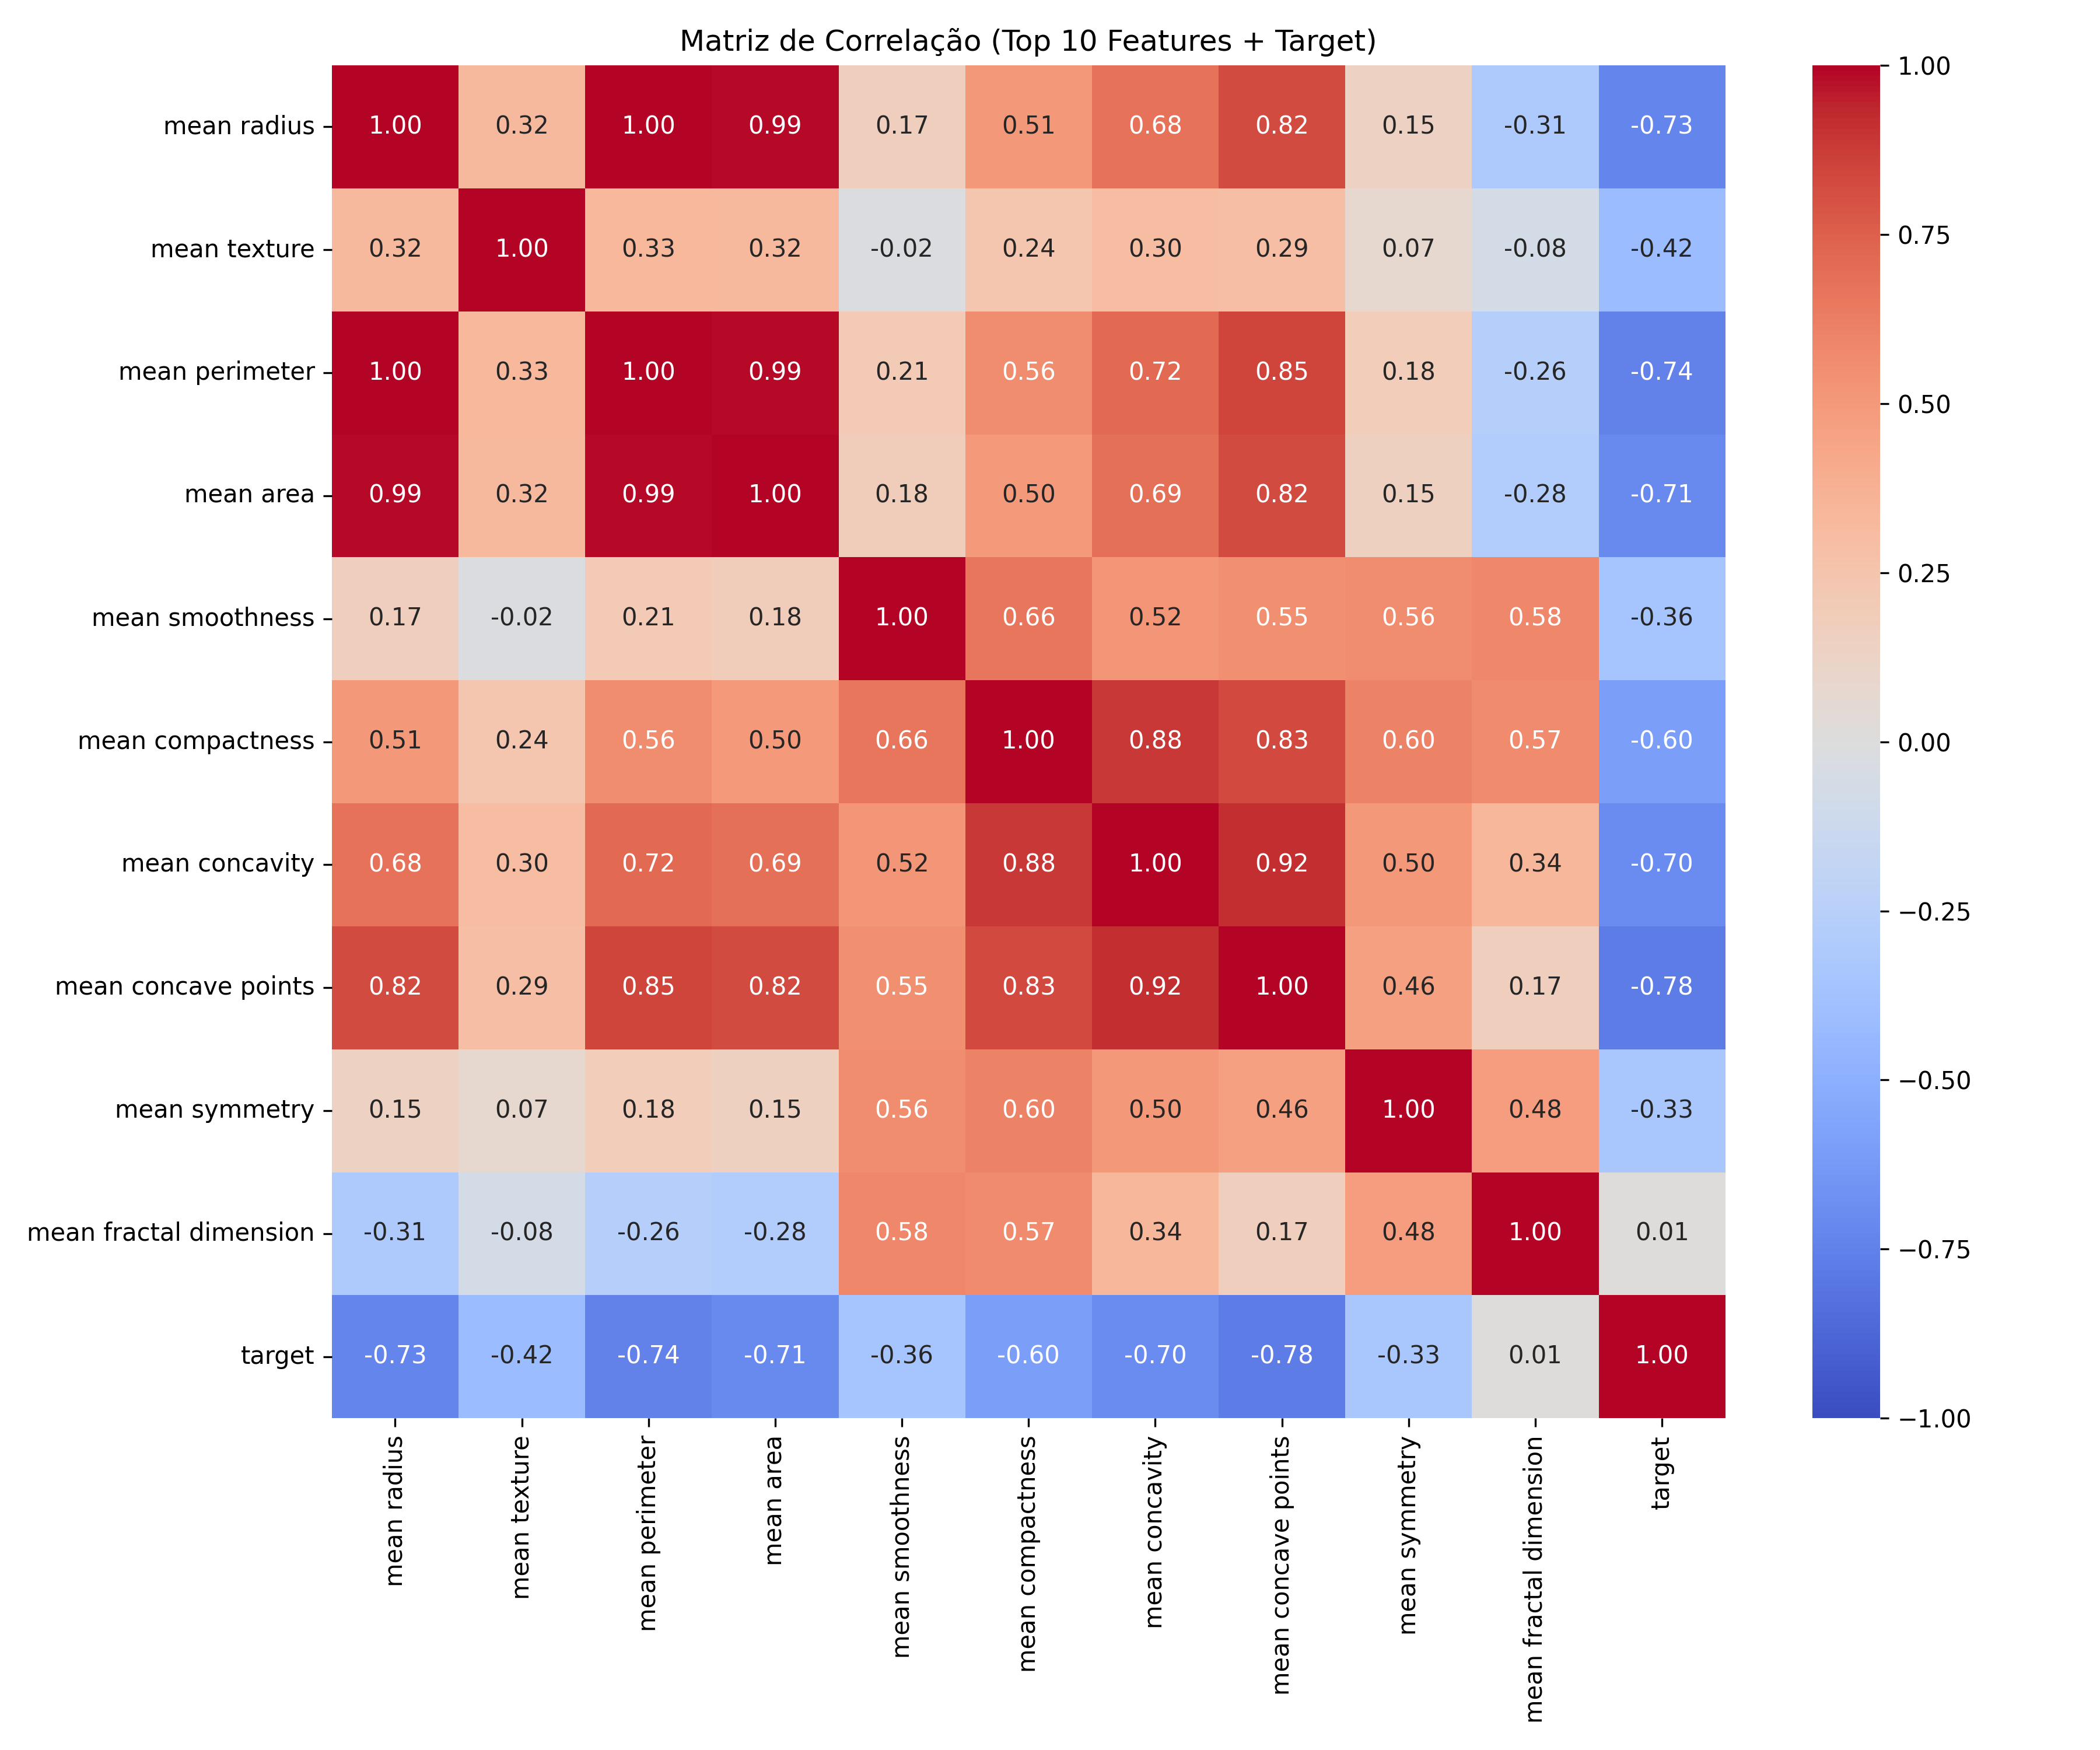
\includegraphics[width=1.1\textwidth]{img/matriz_correlacao.png}
    \caption{Mapa de calor (\textit{Heatmap}) da matriz de correlação das principais características.}
\end{figure}

\subsection{Normalização e Transformação de Escala}
Muitas variáveis neste conjunto de dados operam em grandezas físicas radicalmente distintas. Por exemplo, a \texttt{mean area} pode apresentar valores na casa dos $1000$ (Média $\approx 654.8$), enquanto a \texttt{mean smoothness} e a \texttt{mean symmetry} variam na casa decimal centesimal (Médias $\approx 0.096$ e $\approx 0.181$, respetivamente).

Para resolver esta discrepância, aplicou-se a técnica de \textbf{Padronização} (também conhecida como \textit{Z-score normalization}), implementada através do \texttt{StandardScaler}. Esta técnica reescala os dados para que passem a possuir média zero ($\mu = 0$) e desvio padrão unitário ($\sigma = 1$).

\textbf{Impacto no Desempenho:} A aplicação da Padronização é fundamental e impacta diretamente a convergência e a eficácia de algoritmos de Aprendizado de Máquina. Se esta transformação não fosse aplicada, uma variável com grande magnitude absoluta (como a área) dominaria por completo o cálculo da Função de Custo de algoritmos baseados em descida de gradiente (como Redes Neurais e Regressão Logística) ou de cálculo de distâncias euclidianas (como KNN e SVM), forçando o modelo a ignorar características cruciais que operam em casas decimais (como a suavidade ou a simetria do tumor). Ao padronizar, garante-se que todas as variáveis contribuem de forma equitativa e independente das suas unidades de medida originais.

\end{document}